
% Default to the notebook output style

    


% Inherit from the specified cell style.




    
\documentclass[11pt]{article}

    
    
    \usepackage[T1]{fontenc}
    % Nicer default font (+ math font) than Computer Modern for most use cases
    \usepackage{mathpazo}

    % Basic figure setup, for now with no caption control since it's done
    % automatically by Pandoc (which extracts ![](path) syntax from Markdown).
    \usepackage{graphicx}
    % We will generate all images so they have a width \maxwidth. This means
    % that they will get their normal width if they fit onto the page, but
    % are scaled down if they would overflow the margins.
    \makeatletter
    \def\maxwidth{\ifdim\Gin@nat@width>\linewidth\linewidth
    \else\Gin@nat@width\fi}
    \makeatother
    \let\Oldincludegraphics\includegraphics
    % Set max figure width to be 80% of text width, for now hardcoded.
    \renewcommand{\includegraphics}[1]{\Oldincludegraphics[width=.8\maxwidth]{#1}}
    % Ensure that by default, figures have no caption (until we provide a
    % proper Figure object with a Caption API and a way to capture that
    % in the conversion process - todo).
    \usepackage{caption}
    \DeclareCaptionLabelFormat{nolabel}{}
    \captionsetup{labelformat=nolabel}

    \usepackage{adjustbox} % Used to constrain images to a maximum size 
    \usepackage{xcolor} % Allow colors to be defined
    \usepackage{enumerate} % Needed for markdown enumerations to work
    \usepackage{geometry} % Used to adjust the document margins
    \usepackage{amsmath} % Equations
    \usepackage{amssymb} % Equations
    \usepackage{textcomp} % defines textquotesingle
    % Hack from http://tex.stackexchange.com/a/47451/13684:
    \AtBeginDocument{%
        \def\PYZsq{\textquotesingle}% Upright quotes in Pygmentized code
    }
    \usepackage{upquote} % Upright quotes for verbatim code
    \usepackage{eurosym} % defines \euro
    \usepackage[mathletters]{ucs} % Extended unicode (utf-8) support
    \usepackage[utf8x]{inputenc} % Allow utf-8 characters in the tex document
    \usepackage{fancyvrb} % verbatim replacement that allows latex
    \usepackage{grffile} % extends the file name processing of package graphics 
                         % to support a larger range 
    % The hyperref package gives us a pdf with properly built
    % internal navigation ('pdf bookmarks' for the table of contents,
    % internal cross-reference links, web links for URLs, etc.)
    \usepackage{hyperref}
    \usepackage{longtable} % longtable support required by pandoc >1.10
    \usepackage{booktabs}  % table support for pandoc > 1.12.2
    \usepackage[inline]{enumitem} % IRkernel/repr support (it uses the enumerate* environment)
    \usepackage[normalem]{ulem} % ulem is needed to support strikethroughs (\sout)
                                % normalem makes italics be italics, not underlines
    

    
    
    % Colors for the hyperref package
    \definecolor{urlcolor}{rgb}{0,.145,.698}
    \definecolor{linkcolor}{rgb}{.71,0.21,0.01}
    \definecolor{citecolor}{rgb}{.12,.54,.11}

    % ANSI colors
    \definecolor{ansi-black}{HTML}{3E424D}
    \definecolor{ansi-black-intense}{HTML}{282C36}
    \definecolor{ansi-red}{HTML}{E75C58}
    \definecolor{ansi-red-intense}{HTML}{B22B31}
    \definecolor{ansi-green}{HTML}{00A250}
    \definecolor{ansi-green-intense}{HTML}{007427}
    \definecolor{ansi-yellow}{HTML}{DDB62B}
    \definecolor{ansi-yellow-intense}{HTML}{B27D12}
    \definecolor{ansi-blue}{HTML}{208FFB}
    \definecolor{ansi-blue-intense}{HTML}{0065CA}
    \definecolor{ansi-magenta}{HTML}{D160C4}
    \definecolor{ansi-magenta-intense}{HTML}{A03196}
    \definecolor{ansi-cyan}{HTML}{60C6C8}
    \definecolor{ansi-cyan-intense}{HTML}{258F8F}
    \definecolor{ansi-white}{HTML}{C5C1B4}
    \definecolor{ansi-white-intense}{HTML}{A1A6B2}

    % commands and environments needed by pandoc snippets
    % extracted from the output of `pandoc -s`
    \providecommand{\tightlist}{%
      \setlength{\itemsep}{0pt}\setlength{\parskip}{0pt}}
    \DefineVerbatimEnvironment{Highlighting}{Verbatim}{commandchars=\\\{\}}
    % Add ',fontsize=\small' for more characters per line
    \newenvironment{Shaded}{}{}
    \newcommand{\KeywordTok}[1]{\textcolor[rgb]{0.00,0.44,0.13}{\textbf{{#1}}}}
    \newcommand{\DataTypeTok}[1]{\textcolor[rgb]{0.56,0.13,0.00}{{#1}}}
    \newcommand{\DecValTok}[1]{\textcolor[rgb]{0.25,0.63,0.44}{{#1}}}
    \newcommand{\BaseNTok}[1]{\textcolor[rgb]{0.25,0.63,0.44}{{#1}}}
    \newcommand{\FloatTok}[1]{\textcolor[rgb]{0.25,0.63,0.44}{{#1}}}
    \newcommand{\CharTok}[1]{\textcolor[rgb]{0.25,0.44,0.63}{{#1}}}
    \newcommand{\StringTok}[1]{\textcolor[rgb]{0.25,0.44,0.63}{{#1}}}
    \newcommand{\CommentTok}[1]{\textcolor[rgb]{0.38,0.63,0.69}{\textit{{#1}}}}
    \newcommand{\OtherTok}[1]{\textcolor[rgb]{0.00,0.44,0.13}{{#1}}}
    \newcommand{\AlertTok}[1]{\textcolor[rgb]{1.00,0.00,0.00}{\textbf{{#1}}}}
    \newcommand{\FunctionTok}[1]{\textcolor[rgb]{0.02,0.16,0.49}{{#1}}}
    \newcommand{\RegionMarkerTok}[1]{{#1}}
    \newcommand{\ErrorTok}[1]{\textcolor[rgb]{1.00,0.00,0.00}{\textbf{{#1}}}}
    \newcommand{\NormalTok}[1]{{#1}}
    
    % Additional commands for more recent versions of Pandoc
    \newcommand{\ConstantTok}[1]{\textcolor[rgb]{0.53,0.00,0.00}{{#1}}}
    \newcommand{\SpecialCharTok}[1]{\textcolor[rgb]{0.25,0.44,0.63}{{#1}}}
    \newcommand{\VerbatimStringTok}[1]{\textcolor[rgb]{0.25,0.44,0.63}{{#1}}}
    \newcommand{\SpecialStringTok}[1]{\textcolor[rgb]{0.73,0.40,0.53}{{#1}}}
    \newcommand{\ImportTok}[1]{{#1}}
    \newcommand{\DocumentationTok}[1]{\textcolor[rgb]{0.73,0.13,0.13}{\textit{{#1}}}}
    \newcommand{\AnnotationTok}[1]{\textcolor[rgb]{0.38,0.63,0.69}{\textbf{\textit{{#1}}}}}
    \newcommand{\CommentVarTok}[1]{\textcolor[rgb]{0.38,0.63,0.69}{\textbf{\textit{{#1}}}}}
    \newcommand{\VariableTok}[1]{\textcolor[rgb]{0.10,0.09,0.49}{{#1}}}
    \newcommand{\ControlFlowTok}[1]{\textcolor[rgb]{0.00,0.44,0.13}{\textbf{{#1}}}}
    \newcommand{\OperatorTok}[1]{\textcolor[rgb]{0.40,0.40,0.40}{{#1}}}
    \newcommand{\BuiltInTok}[1]{{#1}}
    \newcommand{\ExtensionTok}[1]{{#1}}
    \newcommand{\PreprocessorTok}[1]{\textcolor[rgb]{0.74,0.48,0.00}{{#1}}}
    \newcommand{\AttributeTok}[1]{\textcolor[rgb]{0.49,0.56,0.16}{{#1}}}
    \newcommand{\InformationTok}[1]{\textcolor[rgb]{0.38,0.63,0.69}{\textbf{\textit{{#1}}}}}
    \newcommand{\WarningTok}[1]{\textcolor[rgb]{0.38,0.63,0.69}{\textbf{\textit{{#1}}}}}
    
    
    % Define a nice break command that doesn't care if a line doesn't already
    % exist.
    \def\br{\hspace*{\fill} \\* }
    % Math Jax compatability definitions
    \def\gt{>}
    \def\lt{<}
    % Document parameters
    \title{Introducci?n al Aprendizaje por Refuerzos}
    
    
    

    % Pygments definitions
    
\makeatletter
\def\PY@reset{\let\PY@it=\relax \let\PY@bf=\relax%
    \let\PY@ul=\relax \let\PY@tc=\relax%
    \let\PY@bc=\relax \let\PY@ff=\relax}
\def\PY@tok#1{\csname PY@tok@#1\endcsname}
\def\PY@toks#1+{\ifx\relax#1\empty\else%
    \PY@tok{#1}\expandafter\PY@toks\fi}
\def\PY@do#1{\PY@bc{\PY@tc{\PY@ul{%
    \PY@it{\PY@bf{\PY@ff{#1}}}}}}}
\def\PY#1#2{\PY@reset\PY@toks#1+\relax+\PY@do{#2}}

\expandafter\def\csname PY@tok@w\endcsname{\def\PY@tc##1{\textcolor[rgb]{0.73,0.73,0.73}{##1}}}
\expandafter\def\csname PY@tok@c\endcsname{\let\PY@it=\textit\def\PY@tc##1{\textcolor[rgb]{0.25,0.50,0.50}{##1}}}
\expandafter\def\csname PY@tok@cp\endcsname{\def\PY@tc##1{\textcolor[rgb]{0.74,0.48,0.00}{##1}}}
\expandafter\def\csname PY@tok@k\endcsname{\let\PY@bf=\textbf\def\PY@tc##1{\textcolor[rgb]{0.00,0.50,0.00}{##1}}}
\expandafter\def\csname PY@tok@kp\endcsname{\def\PY@tc##1{\textcolor[rgb]{0.00,0.50,0.00}{##1}}}
\expandafter\def\csname PY@tok@kt\endcsname{\def\PY@tc##1{\textcolor[rgb]{0.69,0.00,0.25}{##1}}}
\expandafter\def\csname PY@tok@o\endcsname{\def\PY@tc##1{\textcolor[rgb]{0.40,0.40,0.40}{##1}}}
\expandafter\def\csname PY@tok@ow\endcsname{\let\PY@bf=\textbf\def\PY@tc##1{\textcolor[rgb]{0.67,0.13,1.00}{##1}}}
\expandafter\def\csname PY@tok@nb\endcsname{\def\PY@tc##1{\textcolor[rgb]{0.00,0.50,0.00}{##1}}}
\expandafter\def\csname PY@tok@nf\endcsname{\def\PY@tc##1{\textcolor[rgb]{0.00,0.00,1.00}{##1}}}
\expandafter\def\csname PY@tok@nc\endcsname{\let\PY@bf=\textbf\def\PY@tc##1{\textcolor[rgb]{0.00,0.00,1.00}{##1}}}
\expandafter\def\csname PY@tok@nn\endcsname{\let\PY@bf=\textbf\def\PY@tc##1{\textcolor[rgb]{0.00,0.00,1.00}{##1}}}
\expandafter\def\csname PY@tok@ne\endcsname{\let\PY@bf=\textbf\def\PY@tc##1{\textcolor[rgb]{0.82,0.25,0.23}{##1}}}
\expandafter\def\csname PY@tok@nv\endcsname{\def\PY@tc##1{\textcolor[rgb]{0.10,0.09,0.49}{##1}}}
\expandafter\def\csname PY@tok@no\endcsname{\def\PY@tc##1{\textcolor[rgb]{0.53,0.00,0.00}{##1}}}
\expandafter\def\csname PY@tok@nl\endcsname{\def\PY@tc##1{\textcolor[rgb]{0.63,0.63,0.00}{##1}}}
\expandafter\def\csname PY@tok@ni\endcsname{\let\PY@bf=\textbf\def\PY@tc##1{\textcolor[rgb]{0.60,0.60,0.60}{##1}}}
\expandafter\def\csname PY@tok@na\endcsname{\def\PY@tc##1{\textcolor[rgb]{0.49,0.56,0.16}{##1}}}
\expandafter\def\csname PY@tok@nt\endcsname{\let\PY@bf=\textbf\def\PY@tc##1{\textcolor[rgb]{0.00,0.50,0.00}{##1}}}
\expandafter\def\csname PY@tok@nd\endcsname{\def\PY@tc##1{\textcolor[rgb]{0.67,0.13,1.00}{##1}}}
\expandafter\def\csname PY@tok@s\endcsname{\def\PY@tc##1{\textcolor[rgb]{0.73,0.13,0.13}{##1}}}
\expandafter\def\csname PY@tok@sd\endcsname{\let\PY@it=\textit\def\PY@tc##1{\textcolor[rgb]{0.73,0.13,0.13}{##1}}}
\expandafter\def\csname PY@tok@si\endcsname{\let\PY@bf=\textbf\def\PY@tc##1{\textcolor[rgb]{0.73,0.40,0.53}{##1}}}
\expandafter\def\csname PY@tok@se\endcsname{\let\PY@bf=\textbf\def\PY@tc##1{\textcolor[rgb]{0.73,0.40,0.13}{##1}}}
\expandafter\def\csname PY@tok@sr\endcsname{\def\PY@tc##1{\textcolor[rgb]{0.73,0.40,0.53}{##1}}}
\expandafter\def\csname PY@tok@ss\endcsname{\def\PY@tc##1{\textcolor[rgb]{0.10,0.09,0.49}{##1}}}
\expandafter\def\csname PY@tok@sx\endcsname{\def\PY@tc##1{\textcolor[rgb]{0.00,0.50,0.00}{##1}}}
\expandafter\def\csname PY@tok@m\endcsname{\def\PY@tc##1{\textcolor[rgb]{0.40,0.40,0.40}{##1}}}
\expandafter\def\csname PY@tok@gh\endcsname{\let\PY@bf=\textbf\def\PY@tc##1{\textcolor[rgb]{0.00,0.00,0.50}{##1}}}
\expandafter\def\csname PY@tok@gu\endcsname{\let\PY@bf=\textbf\def\PY@tc##1{\textcolor[rgb]{0.50,0.00,0.50}{##1}}}
\expandafter\def\csname PY@tok@gd\endcsname{\def\PY@tc##1{\textcolor[rgb]{0.63,0.00,0.00}{##1}}}
\expandafter\def\csname PY@tok@gi\endcsname{\def\PY@tc##1{\textcolor[rgb]{0.00,0.63,0.00}{##1}}}
\expandafter\def\csname PY@tok@gr\endcsname{\def\PY@tc##1{\textcolor[rgb]{1.00,0.00,0.00}{##1}}}
\expandafter\def\csname PY@tok@ge\endcsname{\let\PY@it=\textit}
\expandafter\def\csname PY@tok@gs\endcsname{\let\PY@bf=\textbf}
\expandafter\def\csname PY@tok@gp\endcsname{\let\PY@bf=\textbf\def\PY@tc##1{\textcolor[rgb]{0.00,0.00,0.50}{##1}}}
\expandafter\def\csname PY@tok@go\endcsname{\def\PY@tc##1{\textcolor[rgb]{0.53,0.53,0.53}{##1}}}
\expandafter\def\csname PY@tok@gt\endcsname{\def\PY@tc##1{\textcolor[rgb]{0.00,0.27,0.87}{##1}}}
\expandafter\def\csname PY@tok@err\endcsname{\def\PY@bc##1{\setlength{\fboxsep}{0pt}\fcolorbox[rgb]{1.00,0.00,0.00}{1,1,1}{\strut ##1}}}
\expandafter\def\csname PY@tok@kc\endcsname{\let\PY@bf=\textbf\def\PY@tc##1{\textcolor[rgb]{0.00,0.50,0.00}{##1}}}
\expandafter\def\csname PY@tok@kd\endcsname{\let\PY@bf=\textbf\def\PY@tc##1{\textcolor[rgb]{0.00,0.50,0.00}{##1}}}
\expandafter\def\csname PY@tok@kn\endcsname{\let\PY@bf=\textbf\def\PY@tc##1{\textcolor[rgb]{0.00,0.50,0.00}{##1}}}
\expandafter\def\csname PY@tok@kr\endcsname{\let\PY@bf=\textbf\def\PY@tc##1{\textcolor[rgb]{0.00,0.50,0.00}{##1}}}
\expandafter\def\csname PY@tok@bp\endcsname{\def\PY@tc##1{\textcolor[rgb]{0.00,0.50,0.00}{##1}}}
\expandafter\def\csname PY@tok@fm\endcsname{\def\PY@tc##1{\textcolor[rgb]{0.00,0.00,1.00}{##1}}}
\expandafter\def\csname PY@tok@vc\endcsname{\def\PY@tc##1{\textcolor[rgb]{0.10,0.09,0.49}{##1}}}
\expandafter\def\csname PY@tok@vg\endcsname{\def\PY@tc##1{\textcolor[rgb]{0.10,0.09,0.49}{##1}}}
\expandafter\def\csname PY@tok@vi\endcsname{\def\PY@tc##1{\textcolor[rgb]{0.10,0.09,0.49}{##1}}}
\expandafter\def\csname PY@tok@vm\endcsname{\def\PY@tc##1{\textcolor[rgb]{0.10,0.09,0.49}{##1}}}
\expandafter\def\csname PY@tok@sa\endcsname{\def\PY@tc##1{\textcolor[rgb]{0.73,0.13,0.13}{##1}}}
\expandafter\def\csname PY@tok@sb\endcsname{\def\PY@tc##1{\textcolor[rgb]{0.73,0.13,0.13}{##1}}}
\expandafter\def\csname PY@tok@sc\endcsname{\def\PY@tc##1{\textcolor[rgb]{0.73,0.13,0.13}{##1}}}
\expandafter\def\csname PY@tok@dl\endcsname{\def\PY@tc##1{\textcolor[rgb]{0.73,0.13,0.13}{##1}}}
\expandafter\def\csname PY@tok@s2\endcsname{\def\PY@tc##1{\textcolor[rgb]{0.73,0.13,0.13}{##1}}}
\expandafter\def\csname PY@tok@sh\endcsname{\def\PY@tc##1{\textcolor[rgb]{0.73,0.13,0.13}{##1}}}
\expandafter\def\csname PY@tok@s1\endcsname{\def\PY@tc##1{\textcolor[rgb]{0.73,0.13,0.13}{##1}}}
\expandafter\def\csname PY@tok@mb\endcsname{\def\PY@tc##1{\textcolor[rgb]{0.40,0.40,0.40}{##1}}}
\expandafter\def\csname PY@tok@mf\endcsname{\def\PY@tc##1{\textcolor[rgb]{0.40,0.40,0.40}{##1}}}
\expandafter\def\csname PY@tok@mh\endcsname{\def\PY@tc##1{\textcolor[rgb]{0.40,0.40,0.40}{##1}}}
\expandafter\def\csname PY@tok@mi\endcsname{\def\PY@tc##1{\textcolor[rgb]{0.40,0.40,0.40}{##1}}}
\expandafter\def\csname PY@tok@il\endcsname{\def\PY@tc##1{\textcolor[rgb]{0.40,0.40,0.40}{##1}}}
\expandafter\def\csname PY@tok@mo\endcsname{\def\PY@tc##1{\textcolor[rgb]{0.40,0.40,0.40}{##1}}}
\expandafter\def\csname PY@tok@ch\endcsname{\let\PY@it=\textit\def\PY@tc##1{\textcolor[rgb]{0.25,0.50,0.50}{##1}}}
\expandafter\def\csname PY@tok@cm\endcsname{\let\PY@it=\textit\def\PY@tc##1{\textcolor[rgb]{0.25,0.50,0.50}{##1}}}
\expandafter\def\csname PY@tok@cpf\endcsname{\let\PY@it=\textit\def\PY@tc##1{\textcolor[rgb]{0.25,0.50,0.50}{##1}}}
\expandafter\def\csname PY@tok@c1\endcsname{\let\PY@it=\textit\def\PY@tc##1{\textcolor[rgb]{0.25,0.50,0.50}{##1}}}
\expandafter\def\csname PY@tok@cs\endcsname{\let\PY@it=\textit\def\PY@tc##1{\textcolor[rgb]{0.25,0.50,0.50}{##1}}}

\def\PYZbs{\char`\\}
\def\PYZus{\char`\_}
\def\PYZob{\char`\{}
\def\PYZcb{\char`\}}
\def\PYZca{\char`\^}
\def\PYZam{\char`\&}
\def\PYZlt{\char`\<}
\def\PYZgt{\char`\>}
\def\PYZsh{\char`\#}
\def\PYZpc{\char`\%}
\def\PYZdl{\char`\$}
\def\PYZhy{\char`\-}
\def\PYZsq{\char`\'}
\def\PYZdq{\char`\"}
\def\PYZti{\char`\~}
% for compatibility with earlier versions
\def\PYZat{@}
\def\PYZlb{[}
\def\PYZrb{]}
\makeatother


    % Exact colors from NB
    \definecolor{incolor}{rgb}{0.0, 0.0, 0.5}
    \definecolor{outcolor}{rgb}{0.545, 0.0, 0.0}



    
    % Prevent overflowing lines due to hard-to-break entities
    \sloppy 
    % Setup hyperref package
    \hypersetup{
      breaklinks=true,  % so long urls are correctly broken across lines
      colorlinks=true,
      urlcolor=urlcolor,
      linkcolor=linkcolor,
      citecolor=citecolor,
      }
    % Slightly bigger margins than the latex defaults
    
    \geometry{verbose,tmargin=1in,bmargin=1in,lmargin=1in,rmargin=1in}
    
    

    \begin{document}
    
    
    \maketitle
    
    

    
    \section{Introducción al Aprendizaje por
Refuerzos}\label{introducciuxf3n-al-aprendizaje-por-refuerzos}

\subsubsection{Curso Aprendizaje por Refuerzos, Diplomatura en Ciencia
de Datos, Aprendizaje Automático y sus
Aplicaciones}\label{curso-aprendizaje-por-refuerzos-diplomatura-en-ciencia-de-datos-aprendizaje-automuxe1tico-y-sus-aplicaciones}

\subsubsection{FaMAF, 2018}\label{famaf-2018}

\paragraph{Agenda Clase 1 Parte 1}\label{agenda-clase-1-parte-1}

\begin{itemize}
\tightlist
\item
  Presentación Docentes
\item
  Introducción. Modelo Agente Entorno. Agente Situado. Arquitectura
  Actor-Crítico.
\item
  Aprendizaje por Refuerzos. Elementos. Ciclo del Aprendizaje por
  Refuerzos. Definición Formal.
\item
  Procesos de Decisión de Markov. Función de Valor. Ecuación de Bellman.
  Optimalidad.
\item
  Aproximaciones al Aprendizaje. Model Free y Model Based.

  \begin{itemize}
  \tightlist
  \item
    Iteración de Política.
  \item
    Iteración de Valor.
  \end{itemize}
\end{itemize}

    \subsection{Docentes}\label{docentes}

\begin{itemize}
\tightlist
\item
  Jorge A. Palombarini
\item
  Juan Cruz Barsce
\item
  Ezequiel Beccaría
\end{itemize}

\subsection{Página y Libro Sutton}\label{puxe1gina-y-libro-sutton}

http://incompleteideas.net/

https://drive.google.com/file/d/1opPSz5AZ\_kVa1uWOdOiveNiBFiEOHjkG/view

    \subsection{Link Slack}\label{link-slack}

https://join.slack.com/t/rldiplodatos/shared\_invite/enQtNDQ5Mjg4OTE1NzQ2LTJjYzk2YTI0MzI2YjhjZjAzNGZkOWQ2ZDg4ZTliYzU4Njg1ODViMDhhNjg5NGFiY2ExODAzM2ZmYzgyNTFlZTY

    \subsection{Introducción: Entidad Inteligente -\textgreater{} Agente
Situado}\label{introducciuxf3n-entidad-inteligente---agente-situado}

\begin{itemize}
\item
  La idea de aprender por interacción con nuestro entorno es quizás la
  primera en aparecer cuando pensamos acerca de la naturaleza del
  aprendizaje.
\item
  Por ejemplo, cuando un niño juega, mueve sus brazos, o mira alrededor,
  no tiene un "maestro" explicito, pero posee una conexion sensorial y
  motora con su entorno.
\item
  El ejercicio de dicha conexión produce información acerca de la
  relación causa-efecto y las consecuencias de las acciones que lleva a
  cabo, y respecto de qué hacer de manera tal de lograr objetivos. Así,
  \emph{aprender por interacción} es una idea fundacional de muchas
  teorías del aprendizaje y la inteligencia.
\item
  En este curso, se explorará un enfoque computacional dirigido por
  objetivos para \emph{aprender por interacción}: el \textbf{Aprendizaje
  por Refuerzos (Reinforcement Learning)}.
\end{itemize}

    \subsection{Agent-Environment
Framework}\label{agent-environment-framework}

\begin{itemize}
\item
  El desarrollo de la inteligencia requiere que la entidad o el agente
  esté situada/o en un entorno \textbf{(Measuring universal
  intelligence: Towards an anytime intelligence test, Hernandez-Orallo
  \& Dowe, Artificial Intelligence, 2010).}
  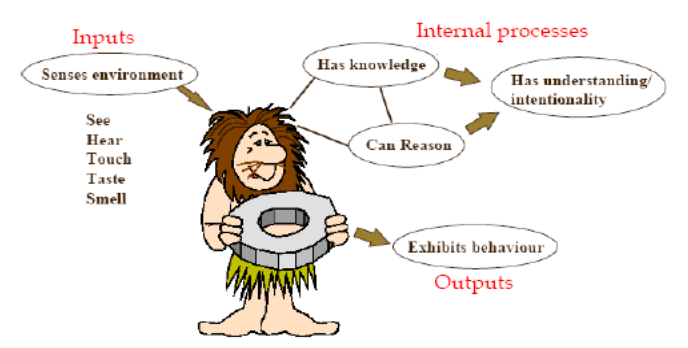
\includegraphics{images/Situated Agent.png}
\item
  El agente y su entorno interactúan a través de la ejecución de
  acciones, observación de estados y señales de reward. La inteligencia
  tendrá efecto sólo si el agente tiene claramente definidos objetivos o
  metas que persigue activamente mientras ocurre la interacción.
  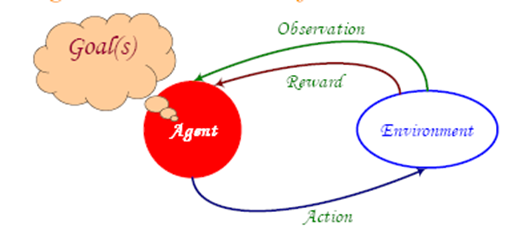
\includegraphics{images/AE Interaction.png}
\end{itemize}

    \subsection{Arquitectura
Actor-Crítico}\label{arquitectura-actor-cruxedtico}

\begin{figure}
\centering
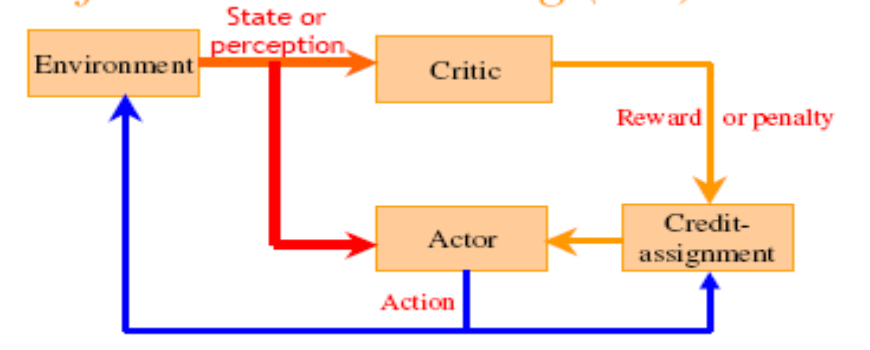
\includegraphics{images/RL Diagram.png}
\caption{}
\end{figure}

    \subsection{Reinforcement Learning}\label{reinforcement-learning}

\begin{itemize}
\item
  \textbf{\emph{Reinforcement learning}} consiste en aprender
  \textbf{que hacer} -mapear situaciones a acciones- de manera tal de
  \textbf{maximizar} una señal numérica de recompensa.
\item
  Al aprendiz no se le especifica cuáles acciones ejecutar, sino que
  debe descubrir a través de \textbf{\emph{prueba y error}} cuáles
  acciones producen la mayor cantidad de recompensa acumulada. En los
  casos más interesantes, las acciones pueden afectar no solo la
  recompensa inmediata, sino solamente el estado, recibiéndose una
  recompensa sólo en algunos estados o bien al final del episodio
  (\textbf{\emph{Delayed-reward}}).
\item
  Se conoce simultaneamente como RL al problema de aprender por
  interacción, a la clase de métodos de solución de dicho problema, y al
  área de la IA que estudia el problema y los métodos de solución.
\item
  El problema de RL puede ser formalizado empleando \textbf{Procesos de
  Decisión de Markov}.
\item
  La toma de decisiones secuencial involucra aprender sobre nuestro
  entorno y elegir acciones que maximizan el retorno esperado. El RL
  computacional, inspirado por estas ideas, las formalizo y produjo un
  impacto importante en robótica, machine learning y neurociencias.
\item
  El Aprendizaje por Refuerzos (RL) consiste en un agente que se
  encuentra en algún estado \(s \in S\) inmerso en un entorno \(E\) y
  toma acciones \(a \in A\) en busca de una meta. El agente puede ser
  modelado formalmente como una función f, que toma un historial de
  interacción como entrada, y devuelve una acción a tomar. Una manera
  conveniente para representar el agente es una medida de probabilidad
  sobre el set A de acciones, en base a un historial de interacción:
  \[ f(a_{n}|s_{1}a_{1} r_{2} s_{2}a_{2}...r_{n}s_{n}) \] que representa
  la probabilidad de la acción a en el ciclo n dado un historial de
  interacción.
\end{itemize}

\begin{figure}
\centering
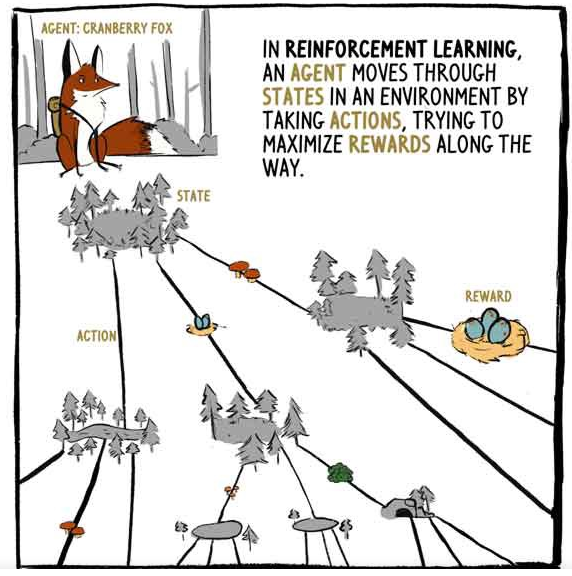
\includegraphics{images/fox-rl.png}
\caption{}
\end{figure}

\begin{itemize}
\item
  Problema RL: \textbf{\emph{¿Cómo el agente produce la distribución de
  probabilidad sobre las acciones?}}
\item
  \textbf{\emph{Dilema de exploración - explotación}}: debido a que el
  Agente no recibe ejemplos de entrenamiento, debe probar alternativas,
  procesar los resultados de sus acciones y modificar su comportamiento
  en algún sentido. ¿Cuándo explotar este conocimiento vs. cuándo probar
  nuevas estrategias?
\end{itemize}

    \subsection{Elementos del Aprendizaje por
Refuerzos}\label{elementos-del-aprendizaje-por-refuerzos}

\begin{figure}
\centering
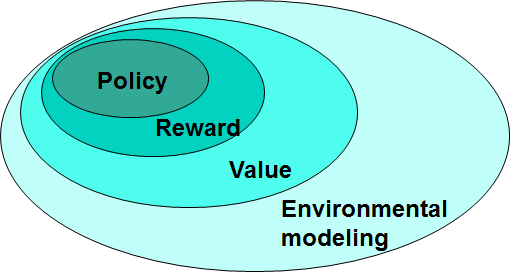
\includegraphics{images/RL Elements.png}
\caption{}
\end{figure}

\begin{itemize}
\tightlist
\item
  \textbf{Policy (Política): }
\end{itemize}

Una política define la manera de comportarse de un agente, en cualquier
momento de tiempo dado. Basicamente, es un mapeo de un estado o
percepción s a una acción a, pudiendo ser estocásticas.

\begin{itemize}
\tightlist
\item
  \textbf{Reward Function (Función de Recompensa)}
\end{itemize}

Define cuantitativamente el objetivo del agente. Es un mapeo de un par
estado-acción a un número real que indica "cuán deseable" es ejecutar
dicha acción en ese estado. Asimismo, el único objetivo del agente es
maximizar la recompensa total que recibe a lo large del tiempo. Cabe
mencionar que, si bien la función de reward no puede ser alterada por el
agente, provee las bases para cambiar la política del mismo.

\begin{itemize}
\tightlist
\item
  \textbf{Value function (Función de Valor)}
\end{itemize}

La función de valor se diferencia de la función de reward en el sentido
de que indica "cuán deseable" es, a largo plazo, ejecutar una acción en
un determinado estado. Así, el valor de un estado s es la cantidad total
de reward que el agente espera obtener a futuro comenzando la
interacción en el estado s.

\begin{itemize}
\tightlist
\item
  \textbf{Environment (Entorno)}
\end{itemize}

El entorno se encuentra constitutido por todo aquel elemento (real o
simulado) que el agente no puede controlar. Es con quién el agente
interactúa a partir de la ejecución de acciones de control.

\subsection{Ciclo del Aprendizaje por
Refuerzos}\label{ciclo-del-aprendizaje-por-refuerzos}

\begin{figure}
\centering
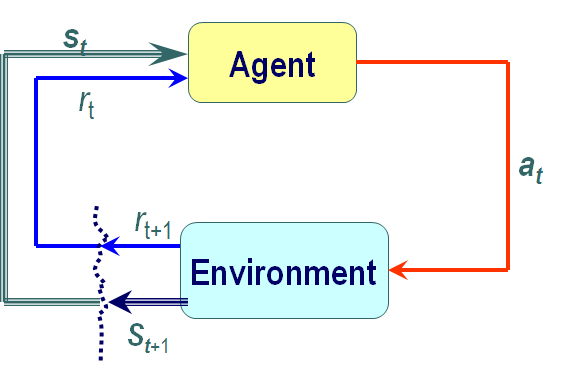
\includegraphics{images/RL Cycle.png}
\caption{}
\end{figure}

    \subsubsection{Definición formal}\label{definiciuxf3n-formal}

\begin{itemize}
\tightlist
\item
  Si el problema de RL dado tiene un conjunto finito de estados y
  acciones y satisface la propiedad de Markov entonces puede definirse
  como un Proceso de Decisión de Markov
\end{itemize}

\begin{equation}
MDPFinito = (S, A, P(.), R(.), γ)
\end{equation}

donde

\[ S = {s_{1}, s_{2}, ..., s_{n}} \] es un conjunto finito de estados.

\begin{figure}
\centering
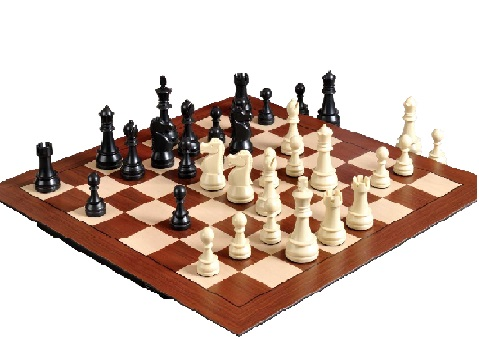
\includegraphics{images/ajedrez-estado.jpg}
\caption{}
\end{figure}

\begin{figure}
\centering
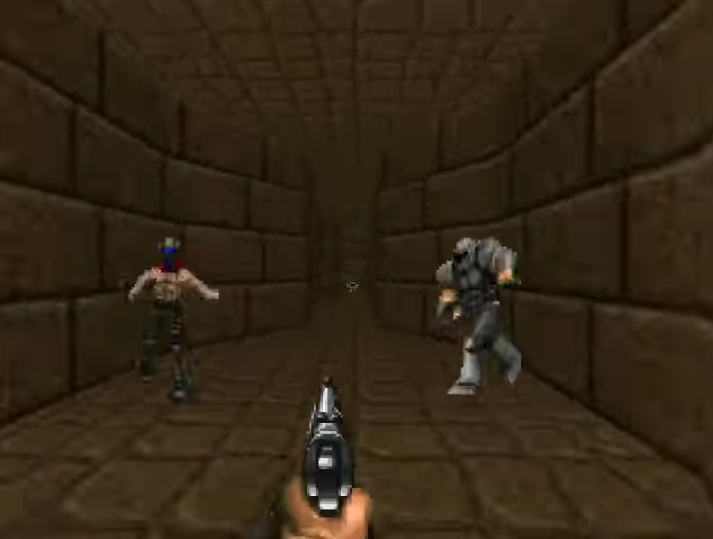
\includegraphics{images/doom-estado.png}
\caption{}
\end{figure}

\[ A = {a_{1}, a_{2}, ..., a_{m}} \] es un conjunto finito de acciones.
\[ P_{a}(s,s') = P(s_{t+1} = s | s_{t} = s, a_{t} = a) \] es la
probabilidad de que la acción a tomada en tiempo t y en estado s lleve
al agente al estado s' en tiempo t+1 \[ R_{a}(s,s') \] es la recompensa
inmediata recibido tras transicionar, luego de tomar la acción a, desde
el estado s al estado s' \[\gamma \in  [0,1]\] es el factor de
descuento, representando la diferencia en la importancia de la
recompensa a corto plazo vs la recompensa a largo plazo.

    \begin{figure}
\centering
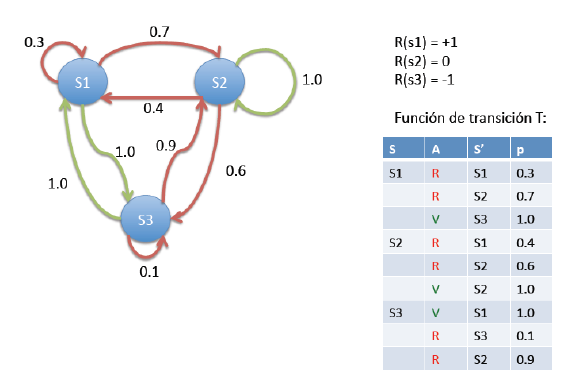
\includegraphics{images/mdp_example.png}
\caption{}
\end{figure}

    \begin{itemize}
\item
  Un episodio (instancia) de este MDP forma una secuencia finita
  \[s_{0}, a_{0}, r_{1}, s_{1}, a_{1}, r_{2}, s_{2}, ... , s_{n-1}, a_{n-1}, r_{n}, s_{n} \]
  donde \[s_{n}\] es un estado final (o n es el tiempo de corte).
\item
  La recompensa total del episodio está dado por
  \[ R = r_{1} + r_{2} + ... + r_{n} \]
\item
  En consecuencia, la recompensa a futuro partiendo del tiempo \(t\)
  está dado por \[R_{t} = r_{t} + r_{t+1} + ... \]
\item
  Hay que considerar que el ambiente es estocástico en la mayor parte de
  los entornos reales y, por tanto, la recompensa suele diverger
  mientras más alejado se encuentre el instante de tiempo considerado.
  Es por esto que se utiliza un parámetro \(γ\) llamado \emph{factor de
  descuento}, para descontar el valor de las recompensas futuras. De
  esta manera,
\end{itemize}

\begin{equation} R_{t} = r_{t} + γr_{t+1} + γ^2r_{t+2} + γ^3r_{t+3} + ... = r_{t} + γ(r_{t+1} + γr_{t+2} + γ^2r_{t+3} ...) = r_{t} + γR_{t+1} \end{equation}

\begin{itemize}
\item
  Si utilizamos \(γ=0\), el agente priorizará sólo la recompensa
  inmediata, mientras que \(\gamma=1\) hará que considere todas los
  recompensas de la misma manera, independientemente del momento en
  donde las reciba. 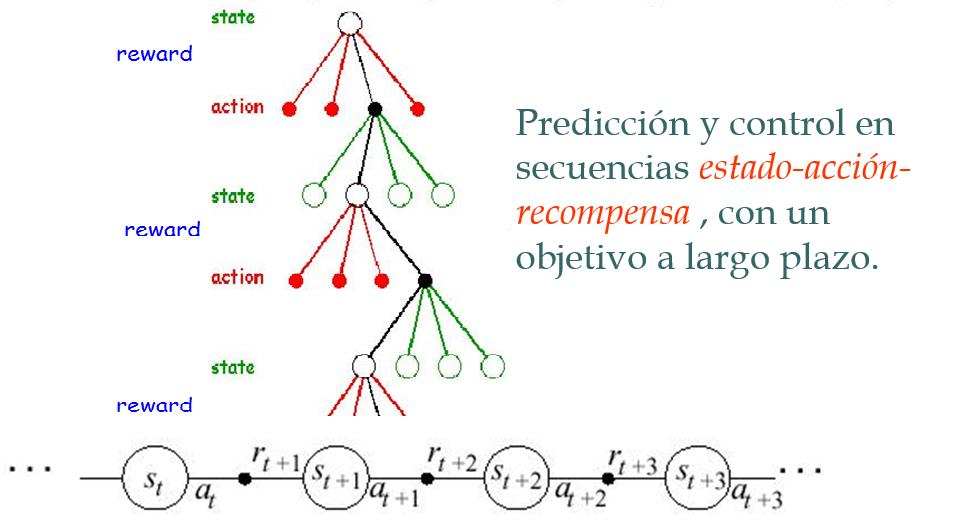
\includegraphics{images/RL Problem Statement.png}
\item
  Dado un Proceso de Decisión de Markov, una Política (determiniística)
  es una función \(\pi\) que a partir de un estado \(s \in S\), devuelve
  como resultado una acción \(a \in A\). Una política estocástica
  devuelve, para un estado \(s\) y una acción \(a\), una probabilidad.
\end{itemize}

    \subsection{Procesos de Decisión de
Markov}\label{procesos-de-decisiuxf3n-de-markov}

\subsubsection{Función de Valor}\label{funciuxf3n-de-valor}

\begin{itemize}
\tightlist
\item
  El valor de un estado es el retorno esperado por el agente, comenzando
  la interacción en dicho estado, dependiendo de la política ejecutada
  por el agente.
\end{itemize}

\begin{figure}
\centering
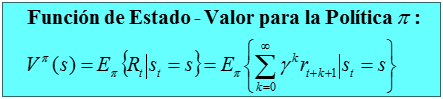
\includegraphics{images/Funcion de Estado Valor.png}
\caption{}
\end{figure}

\begin{itemize}
\tightlist
\item
  El valor de la ejecución de una acción en un estado es el retorno
  esperado por el agente, comenzando la interacción en dicho estado a
  partir de la ejecución de dicha acción, dependiendo de la política
  ejecutada por el agente.
\end{itemize}

\begin{figure}
\centering
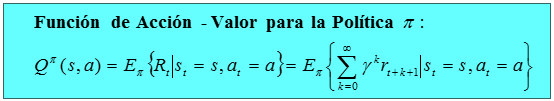
\includegraphics{images/Funcion de Accion Valor.png}
\caption{}
\end{figure}

Una propiedad fundamental de las funciones de valor es que satisfacen
ciertas propiedades recursivas. Para cualquier política π y cualquier
estado s, V(s) y Q(s,a) pueden ser definidas recursivamente en términos
de la denominada \emph{Ecuación de Bellman} ** (Bellman, 1957) **

    \subsubsection{Ecuación de Bellman}\label{ecuaciuxf3n-de-bellman}

\begin{itemize}
\tightlist
\item
  La idea básica es:
\end{itemize}

\begin{figure}
\centering
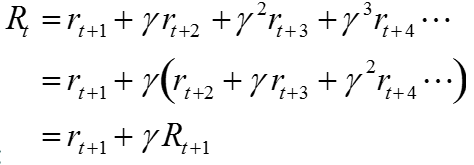
\includegraphics{images/Retorno.png}
\caption{}
\end{figure}

\begin{itemize}
\tightlist
\item
  Entonces,
\end{itemize}

\begin{figure}
\centering
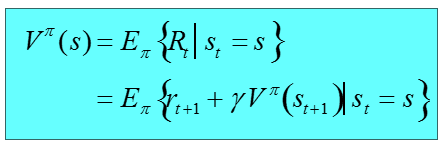
\includegraphics{images/Retorno - Valor.png}
\caption{}
\end{figure}

\begin{itemize}
\tightlist
\item
  O, sin el operador de valor esperado:
\end{itemize}

\begin{figure}
\centering
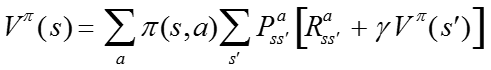
\includegraphics{images/Bellman Equation.png}
\caption{}
\end{figure}

La ecuación anterior refleja el hecho de que el valor de un estado se
encuentra definido en términos de la recompensa inmediata y los valores
de los estados siguientes ponderados en función de las probabilidades de
transición, y adicionalmente un factor de descuento.

    \subsubsection{Ecuación de Optimalidad de
Bellman}\label{ecuaciuxf3n-de-optimalidad-de-bellman}

La Ecuación de Optimalidad de Bellman refleja el hecho de que el Valor
de un estado bajo la política óptima debe ser igual al retorno esperado
para la mejor acción en dicho estado:

\begin{figure}
\centering
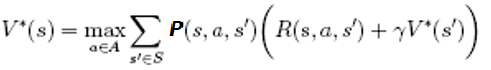
\includegraphics{images/Ecuacion de Optimalidad Valor.png}
\caption{}
\end{figure}

Al mismo tiempo, la acción óptima para un estado s dada la función de
valor, puede obtenerse mediante:

\begin{figure}
\centering
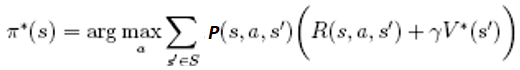
\includegraphics{images/Accion Optima.png}
\caption{}
\end{figure}

La política anterior se denomina \textbf{Política Greedy}, dado que
selecciona la mejor acción para cada estado, teniendo en cuenta la
función de valor V(s). De manera análoga, la función de acción-valor
óptima puede expresarse como:

\begin{figure}
\centering
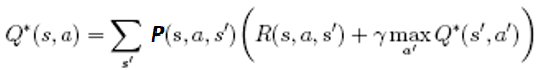
\includegraphics{images/Accion Valor Optima.png}
\caption{}
\end{figure}

    \subsection{Aproximaciones para el aprendizaje de V y Q mediante
Soluciones
Tabulares}\label{aproximaciones-para-el-aprendizaje-de-v-y-q-mediante-soluciones-tabulares}

\begin{figure}
\centering
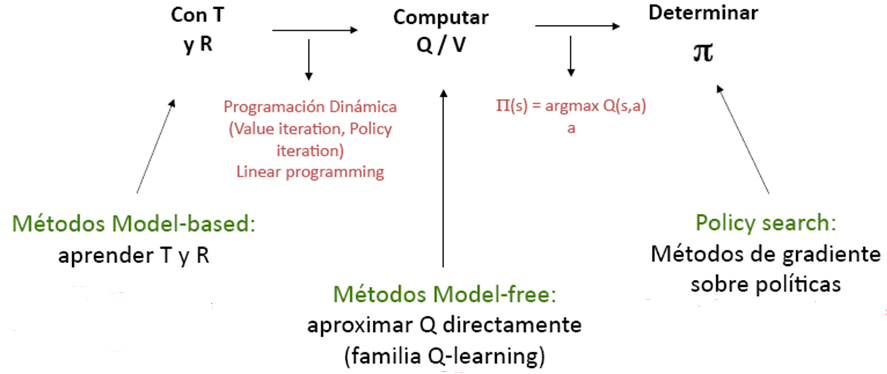
\includegraphics{images/Aproximaciones al aprendizaje.png}
\caption{}
\end{figure}

\subsubsection{Model Based vs. Model
Free}\label{model-based-vs.-model-free}

\begin{itemize}
\item
  Model-free aprende Q/V directamente y presenta muy baja complejidad
  computacional.
\item
  Model-based aprende T y R y usa un algoritmo de planning para
  encontrar la política. Uso eficiente de los datos/experiencia. Alto
  costo computacional.
\end{itemize}

    \subsubsection{Programación Dinámica: Iteración de Valor e Iteración de
Política (Model
Based)}\label{programaciuxf3n-dinuxe1mica-iteraciuxf3n-de-valor-e-iteraciuxf3n-de-poluxedtica-model-based}

\paragraph{Iteración de Valor}\label{iteraciuxf3n-de-valor}

\begin{figure}
\centering
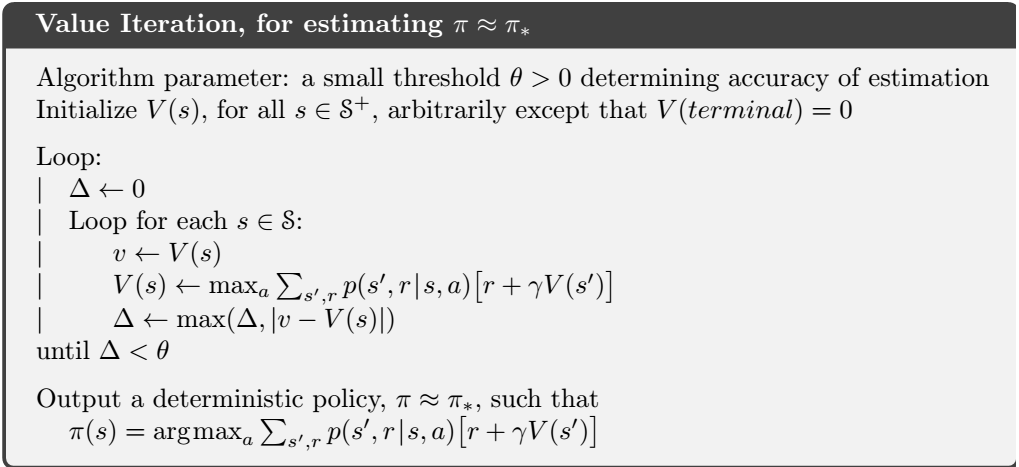
\includegraphics{images/Iteracion de Valor.png}
\caption{}
\end{figure}

\paragraph{Iteración de Política}\label{iteraciuxf3n-de-poluxedtica}

\begin{figure}
\centering
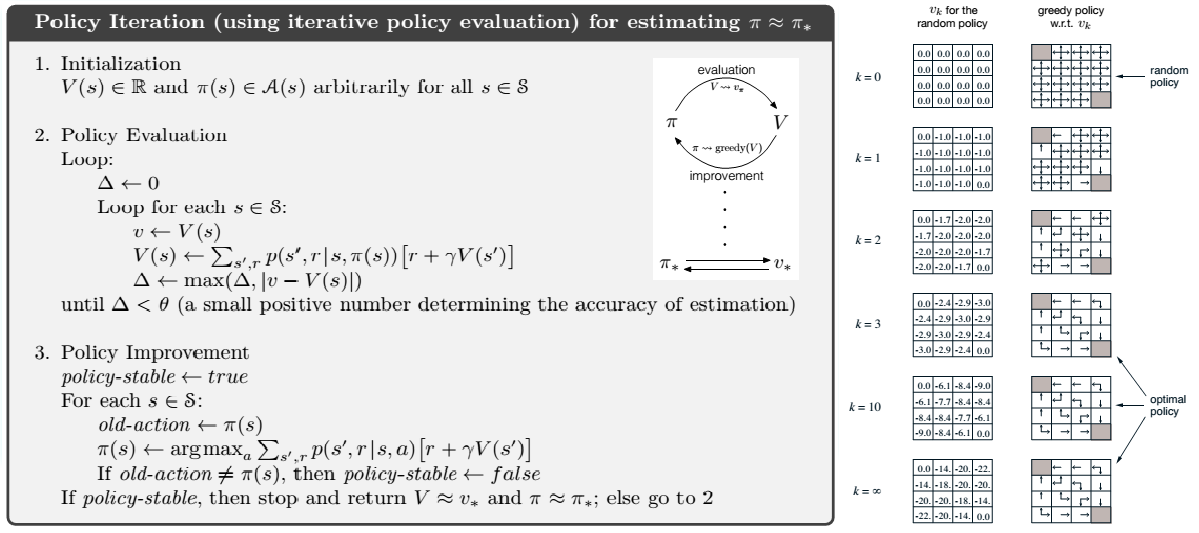
\includegraphics{images/Iteracion de Politica.png}
\caption{}
\end{figure}


    % Add a bibliography block to the postdoc
    
    
    
    \end{document}
